% \subsection{Description}

In a first step, the behavior of the fibre-embedding epoxy matrix is investigated. Matrix cracking is a dominating mechanism for the failure behavior of the overall FRP material and is most likely to cause other phenomena in the course of damage evolution \cite{KrauseD2016}. Therefore, tensile material tests are performed and evaluated on bulk LY564 epoxy resin tensile specimen, as shown in \autoref{fig:Exp:Tension}. The goal is to describe the individual component material properties and failure patterns before application in a more complex structure as shown in \autoref{fig:Exp:MatrixFailure}.

\begin{figure}[htbp]
  \begin{subfigure}{0.3\linewidth}
    \centering
    %\includegraphics[width=\linewidth,height=9cm,keepaspectratio]{../../Material/Figures/DSC_14001_c}
    \includegraphics[width=\linewidth,height=9cm,keepaspectratio]{DSC_14001_c}
    \caption{Static test rig}
    \label{fig:Exp:Tension:TestRig}
  \end{subfigure}%
  \hfill
  \begin{subfigure}{0.69\linewidth}
    \centering
%     \vspace{2ex}

    %\pgfplotstableread[col sep=comma]{Data/Exp_Stress-Strain_LY564_1K-150-mittel.csv}{\loadedtable}
    
    \tikzexternalenable
    \tikzsetnextfilename{Exp_Stress-Strain_LY564_1K-150-mittel}
    \begin{tikzpicture}
      \begin{axis}[
          axis lines=middle,
          width=\linewidth,
          height=5cm,
          xmin=0,
          xmin=0,
          xlabel={Strain $[\si{\percent}]$},
          ylabel={Stress $[\si{\mega\pascal}]$},
%           x label style={at={(axis description cs:0.5,-0.15)},anchor=north},
%           y label style={at={(axis description cs:-0.075,.5)},rotate=90,anchor=south},
          legend style={at={(1.0,0.5)},anchor=east},
        ]
          %\addplot+[black,no marks] table[x=Strain, y=Stress] {\loadedtable};
          \addplot+[lightgray,dash dot,no marks] table[x=Strain, y=Stress, col sep=comma] {../../Material/Data/Tests/Exp_Stress-Strain_LY564_1K-130-mittel.csv};
          \addlegendentry{Cure cycle 1}
          \addplot+[gray,solid,no marks] table[x=Strain, y=Stress, col sep=comma] {../../Material/Data/Tests/Exp_Stress-Strain_LY564_1K-150-mittel.csv};
          \addlegendentry{Cure cycle 2}
          \addplot+[black,dashed,no marks] table[x=Strain, y=Stress, col sep=comma] {../../Material/Data/Tests/Exp_Stress-Strain_LY564_3K-150-mittel.csv};
          \addlegendentry{Cure cycle 3}
      \end{axis}
    \end{tikzpicture}
    \tikzexternaldisable
%     \includegraphics[width=\linewidth,height=4cm,keepaspectratio]{Figures/1K_150_02_c}
    \caption{Effective LY564 stress-strain curve}
    \label{fig:Exp:Tension:StressStrain}
    
    
    %\includegraphics[width=\linewidth,height=4cm,keepaspectratio]{../../Material/Figures/1K_150_02_c}
    \includegraphics[width=\linewidth,height=4cm,keepaspectratio]{1K_150_02_c}
    \caption{Fracture plane micrograph}
    \label{fig:Exp:Tension:Fracture:Micrograph}
  \end{subfigure}%
  \caption{Bulk resin tensile test}
  \label{fig:Exp:Tension}
\end{figure}